\chapter{Identification of Transfer Function of a Single Board Heater System through Ramp Response Experiment}\label{chap2}
The aim of this experiment is to perform ramp test on the Single Board Heater System and to identify the 
system transfer function using ramp response data. The target group is anyone who has basic knowledge of control engineering.
\section{About this experiment}

\begin{figure}
\centering
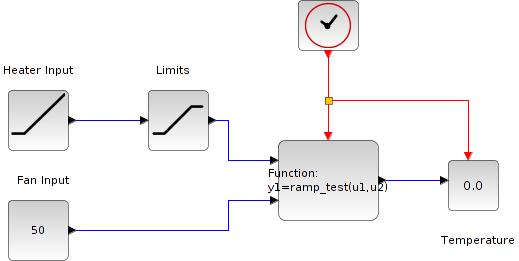
\includegraphics[width=0.7\linewidth]{Ramp-test_manual/ramp_test.jpg}
\caption{Xcos for ramp test experiment}
\label{Xcos_rt}
\end{figure} 
We have used Scilab 5.3.3 and Xcos for sending and receiving data. This interface is shown in figure \ref{Xcos_rt}. 
Heater current and fan speed are the two inputs to the SBHS system. They are given in percentage of maximum output. 
These inputs can be varied through the Xcos interface by setting the properties of the input blocks in Xcos. 
The data acquired in the process is stored in the local drive and is available to the user for further analysis.
\section{Theory}
Identification of the transfer function of a system is important as it helps us model the physical system 
mathematically. Once the transfer function is obtained, one can find out the response of the system to various inputs
without actually applying them to the system.\\
Consider the standard first order transfer function given below
\begin{align}
G(s) &= \frac{ C(s)}{ R(s)}\\ 
G(s)&=\frac K{\tau s+1}\\               
\intertext{Combining the previous two equations, we get}
C(s)  &= K \left\{\frac {R(s)}{\tau s + 1}\right\}\label{fotf}
\intertext{Let us consider the case of giving a ramp input to this first order system. 
The Laplace transform of a ramp function with slope = $\upsilonup$ is $ \frac \upsilonup {s^2}$. 
Substituting $ R(s) = \frac \upsilonup {s^2}$ in equation \ref{fotf}, we obtain}
C(s) & =  \frac K{\tau s + 1}\frac \upsilonup {s^2}\\
&= \frac A{s} + \frac B{s^2} +\frac C{\tau s + 1}\\
\intertext{Solving $C(s)$ using Heaviside expansion approach, we get}
C(s) &= K\upsilonup \left\{\frac1{s^2} -  \frac \tau s + \frac {\tau^2}{\tau s + 1}\right\}\label{Heaviside}\\
\intertext{Taking the Inverse Laplace transform of the above equation, we get}
c(t)&= K\upsilonup \left\{t -\tau   + \tau e^{\frac {-t}\tau }\right\}\label{ct} \\
\intertext{The difference between the reference and output signal is the error signal $e(t)$. Therefore,}
e(t)&= r(t) - c(t)\\
e(t)&= K\upsilonup t - K\upsilonup t + K\upsilonup \tau  - K\upsilonup \tau e^\frac {-t}\tau   \\
e(t)&= K\upsilonup \tau (1 - e^{\frac {-t}\tau})\label{et}\\
\intertext{Normalizing equation \ref{et} for $t>>\tau$, we get}
e(t) &= \tau
\end{align}
This means that the error in following the ramp input is equal to $\tau$ for 
large value of $t$ \cite{ogt05}. Hence, smaller the time constant $\tau$, smaller the steady state error.

\section{Conducting Step Test on SBHS locally}
The detailed procedure to perform a local experiment is explained in Chapter\ref{sercomm}. A summary of the same is provided in section \ref{local-summary} It is same for this section with following changes.

\begin{enumerate}
\item Step1: The working directory is {\tt  Ramp\_test}
\item Step2: Same
\item Step3: Same
\item Step4: Same
\item Step5: Load ramp test function by executing command\\ {\tt exec<space>ramp\_test.sci}
\item Step6: Load Xcos code for ramp test using the command\\ {\tt exec<space>ramp\_test.xcos}
\item Step7: Same
\end{enumerate}

\section{Conducting Step Test on SBHS, virtually}
The steps for conducting a step test experiment virtually is exactly same as explained in section \ref{vlabsexpt}.

\section{Procedure to perform Ramp Test}
Follow the procedure explained in section \ref{scilab_sbhs}.
\begin{enumerate}
 \item Change the Scilab working directory to {\tt Ramp\_Test} folder.
 \item Execute the code {\tt ramp\_test.sci} instead of {\tt step\_test.sci}. 
 \item Open the Xcos file {\tt ramp\_test.xcos}. Give a ramp input to the system with some value for slope. For this 
 experiment, we have chosen slope = $0.1$.
 \item Double click on the ramp input block labled as ``Heater input''. Change the following values in the respective 
 fields- slope = 0.1, start time = 200, initial output = 20.
\item Keep the fan constant at 100.
\end{enumerate}
% Note that the value of heater current will not exceed 40 PWM units due to the use of limit blocks. The Xcos code, on execution,
% may warn you with a message saying ``No continuous-time states. Thresholds are ignored''. Ignore the message by clicking on OK 
% button.
\begin{figure}
\centering
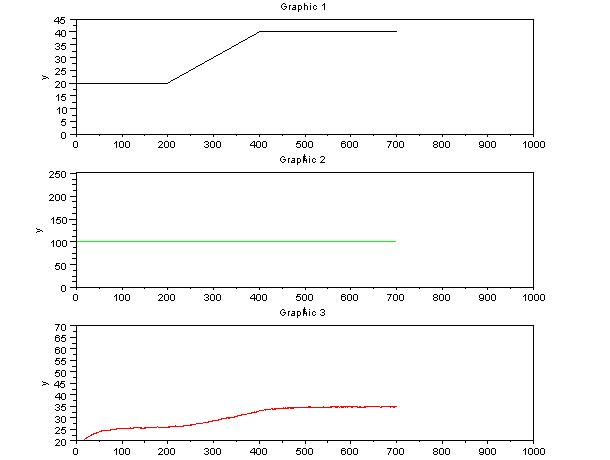
\includegraphics[width=\linewidth]{Ramp-test_manual/ramp_plot.jpg}
\caption{Screen shot of ramp test experiment}
\end{figure}

\begin{table}
\begin{verbatim}
 0.000E+00  0.100E+02  0.100E+03  0.216E+02
 0.100E+00  0.100E+02  0.100E+03  0.216E+02
.
.
 0.251E+03  0.300E+02  0.100E+03  0.291E+02
 0.251E+03  0.300E+02  0.100E+03  0.291E+02
\end{verbatim}
\caption{Ramp data obtained after performing the ramp test}
\label{Rampdata}
\end{table}
The first column of table \ref{Rampdata} denotes samples. 
The second column denotes heater in percentage. The third column denotes the fan. 
It has been held constant at 100 units. The last column denotes the plate temperature.

\section{Ramp Test Analysis}
After completing the ramp test experiment, let us do the analysis. 
\begin{enumerate}
 \item Change the directory to {\tt Ramp\_Analysis}.
 \item Execute the file {\tt ramp.sce}. 
\end{enumerate}
On executing this file, you get the values of Kp, tau and Kp approx and tau approx on the Scilab plot. 
You will also get a plot of the ramp response calculated using the equation \ref{ct} for Kp and tau values.
\begin{figure}[h]
	\centering
		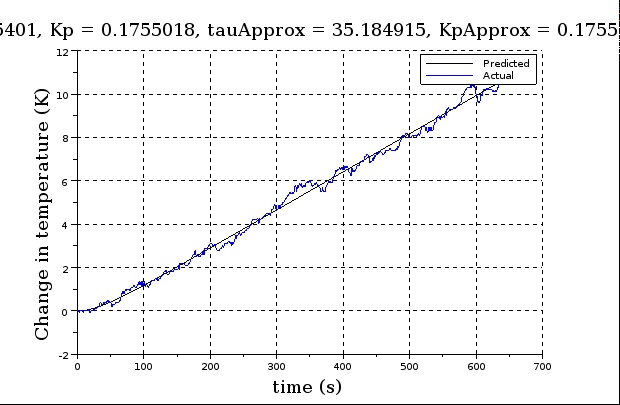
\includegraphics[width=\linewidth]{Ramp-test_manual/ramp_analysis.jpg}
	\caption{Ramp response for Kp and tau}
	\label{fig:fit_curve_ramp}
\end{figure}

\section{Discussion}
We summarize our findings now. The experiment has been performed by varying the heater current and keeping the fan 
speed constant. However, the user is encouraged to experiment using different combinations of fan speed 
and heater current. Negative ramp can also be used to make the experiment more informative. 
It is not necessary to keep a particular input constant. For example, you can try giving a step input to the 
disturbance signal, i.e., the fan input. The system can also be treated as a second order system. This consideration 
is necessary as it increases the accuracy of the acquired transfer function \cite{kmm09}.
\section{Conducting ramp test on SBHS, virtually}
The step by step procedure for conducting an experiment virtually is explained in section \ref{vlabsexpt}. 
\begin{enumerate}
 \item Go to {\tt virtual} folder and then {\tt RampTest} directory
 \item Execute {\tt ramptest.sce}
 \item Perform ramp test analysis by executing {\tt ramp\_virtual.sce} under {\tt Ramp\_Analysis} directory
\end{enumerate}

The necessary codes are listed in the section \ref{rampcodes}.
\end{document}

###################################
\section{Scilab Code}\label{rampcodes}
\begin{code}
\ccaption{ramp\_test.sci}{\ttfamily ramp\_test.sci}
\lstinputlisting{Scilab/local/Ramp_Test/ramp_test.sci}
\end{code}

\begin{code}
\ccaption{label.sci}{\ttfamily label.sci}
\lstinputlisting{Scilab/local/Ramp_Analysis/label.sci}
\end{code}

\begin{code}
\ccaption{cost.sci}{\ttfamily cost.sci}
\lstinputlisting{Scilab/local/Ramp_Analysis/cost.sci}
\end{code}

\begin{code}
\ccaption{cost\_approx.sci}{\ttfamily cost\_approx.sci}
\lstinputlisting{Scilab/local/Ramp_Analysis/cost_approx.sci}
\end{code}

\begin{code}
\ccaption{ramptest.sci}{\ttfamily ramptest.sci}
\lstinputlisting{Scilab/virtual/RampTest/ramptest.sci}
\end{code}

\begin{code}
\ccaption{ramptest.sce}{\ttfamily ramptest.sce}
\lstinputlisting{Scilab/virtual/RampTest/ramptest.sce}
\end{code}

\begin{code}
\ccaption{ramp\_virtual.sce}{\ttfamily ramp\_virtual.sce}
\lstinputlisting{Scilab/virtual/Ramp_Analysis/ramp_virtual.sce}
\end{code}


%\bibliography{New} % Adding References
